

%\begin{frame}
%\frametitle{Wer entwickelt Linux?}
%\begin{figure}
%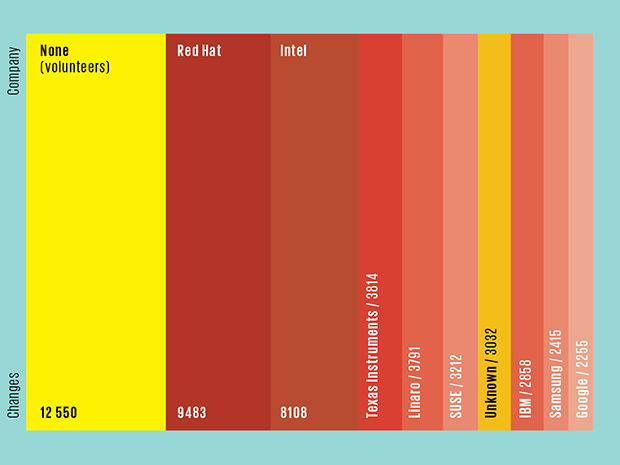
\includegraphics[scale=0.4]{resources/linuxdev.jpg}
%\end{figure}
%http://www.extremetech.com/wp-content/uploads/2014/02/02DataFlowBills3-1390852937757.jpg
%\end{frame}

\begin{frame}
\frametitle{Free vs. OS vs. Kostenlos}
\begin{figure}
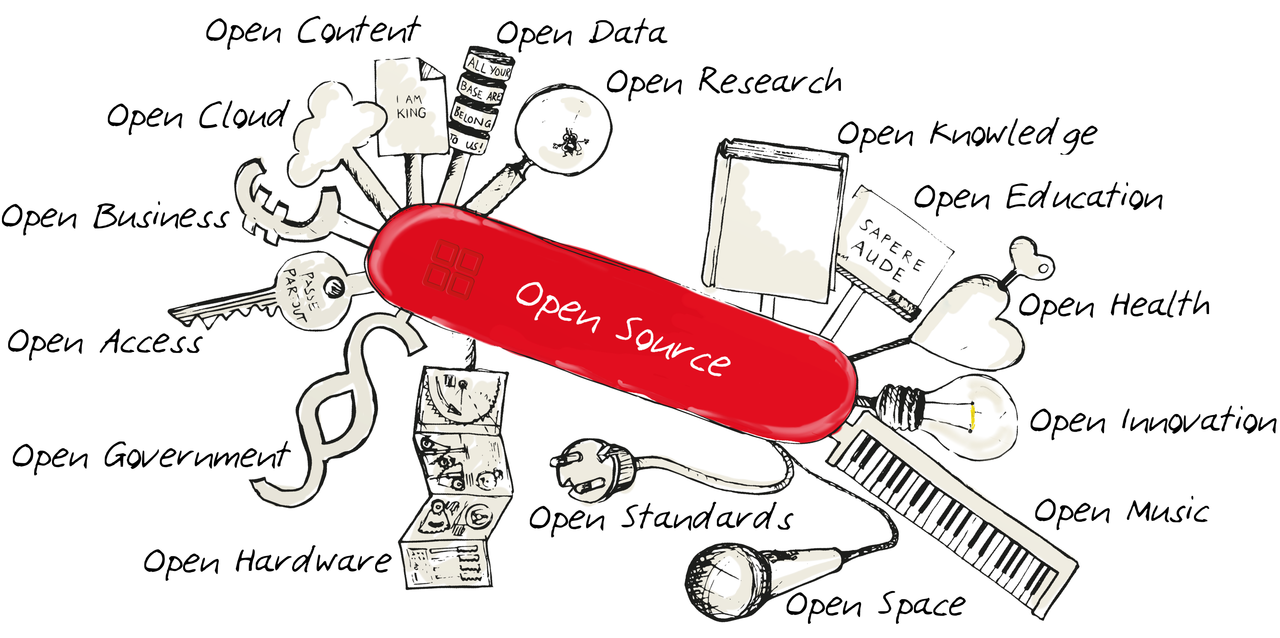
\includegraphics[scale=0.5]{resources/open_swiss_knife.png}
\end{figure}
%Open-Source beschränkt sich nicht nur auf Software
\begin{itemize}
	\item Open-Source == Freies Wissen
	%open source ist denkweise...Wissen soll für alle frei sein
	\item Open-Source Software == Software mit frei zugänglichem Quellcode
	\item Free Software:
	\begin{itemize}
		\item 1. Freiheit der Kontrolle über Software
		%totale Kontrolle über alle Aspekte der Software: Analyse und Änderung. Quellcode muss nicht erhalten werden
		\item 2. Soziale Freiheit der Kolaboration
		%Verbreitung des Quellcodes. Auch kommerzielle Tätigkeiten dürfen angeboten werden
	\end{itemize}
	\item Kostenlose Software (Freeware) == Programmierer verzichtet auf Nutzungsvergütung
	%Freeware Nutzung wird eingeräumt, Änderung allerdings nicht
	%https://de.wikipedia.org/wiki/Datei:121212_2_OpenSwissKnife.png
\end{itemize}

%\footnote{https://de.wikipedia.org/w/index.php?search=kostenlose+Software&title=Spezial$%$3ASuche&fulltext=Volltext}
\end{frame}

\begin{frame}
	\Huge Warum ist Open-Source cool?
\end{frame}

\begin{frame}
	\centering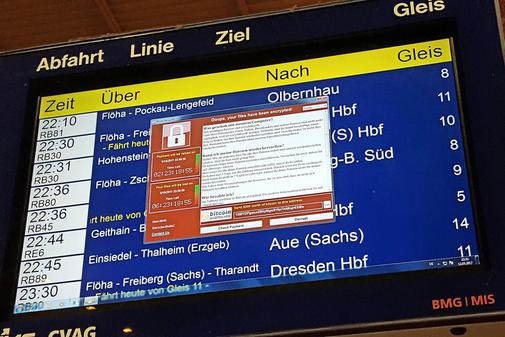
\includegraphics[scale=1.7]{resources/wannacrydb.jpg}
\end{frame}

\begin{frame}
\frametitle{Warum ist Open-Source cool?}
\begin{figure}

\includegraphics[scale=0.4]{resources/att.jpg}
\end{figure}
\begin{itemize}
	\item Fehlerbehebung durch Community
	%Bug Hunting
	\item Schwachstellen und potentielle Angriffsstellen werden erkannt
	%Zero-Date exploits, Backdoors
	\item Kontrolle bzgl. unerwünschter Nebenfunktionen
	%Funktionen zur Überwachung oder zur Erstellung von Hintertüren
\end{itemize}
%\footnote{https://www.bing.com/images/search?q=open+source+meme&view=detailv2&&id=3CEEA01A1F60BB879267791D1040EEB7081F26B2&selectedIndex=101&ccid=0j9v2qqY&simid=607986818429160812&thid=OIP.ee0ac8a908656d52412286fa1abe398f&ajaxhis+t=0}
\end{frame}


\begin{frame}
\frametitle{Linux - Motivation}

\begin{tabular}{cl}
	\begin{tabular}{c}
		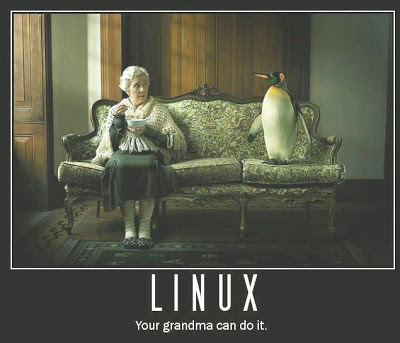
\includegraphics[scale=0.35]{resources/grandmaLinux.jpg}
	\end{tabular}
	& \begin{tabular}{l}
		\parbox{0.5\textwidth}{\begin{itemize}
	\item Linux ist überall
	\begin{itemize}
		\item Server
		\item Arbeitsplatz
		\item Smartphone
	\end{itemize}
	\item Linux ist einfach
	\begin{itemize}
		\item Simple Oberfläche
		\item Stabiles System
		\item Gleiche Funktionalität wie andere Systeme
	\end{itemize}
	%https://2.bp.blogspot.com/_UqUwVPikChs/TFq5scy4dVI/AAAAAAAAOiM/tDuYjZGTSgY/s1600/GrandmaLinux.jpg
\end{itemize}}
	\end{tabular}

\end{tabular}
\end{frame}

\begin{frame}
\frametitle{Was ist Linux?}
\begin{figure}

\includegraphics[scale=0.17]{resources/tux.png}
\end{figure}
\begin{itemize}
	\item Free and Open-Source Mehrbenutzer-Betriebssystem
	\item Basiert auf dem Linux-Kernel
	%von Linus Torvalds für x86 architecture entwickelt
	%Kernel ist Schnittstelle zwischen Software und Hardware
	%Geschrieben in C
	\item Projekt wird unterstützt von Unternehmen, Non-Profit-Organisationen und vielen Freiwilligen
	\item Linux-Distro fasst Kernel und unterschiedliche Software zusammen
	%https://upload.wikimedia.org/wikipedia/commons/a/af/Tux.png
\end{itemize}
\end{frame}

%\begin{frame}
%\frametitle{Was bietet Linux?}
%\begin{figure}
%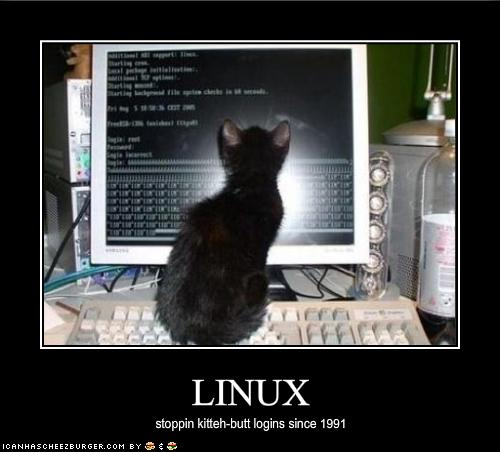
\includegraphics[scale=0.33]{resources/kitteh.jpg}
%\end{figure}
%\begin{itemize}
%	\item Sicher
%	\item Modifizierbar
%	\item Kostenlos
%\end{itemize}
%\footnote{http://danlynch.org/wp-content/uploads/2009/04/funny-pictures-your-kitten-uses-linux.jpg}
%\end{frame}

%\begin{frame}
%\frametitle{Was macht Linux sicher?}
%\begin{figure}
%
\includegraphics[scale=0.3]{resources/infosec.jpg}
%\end{figure}
%\begin{itemize}
%	\item Tausende von Entwicklern prüfen den Code auf Fehler
%	\item Große Firmen haben Teams von ca. 10-30 Leuten 
%	\begin{itemize}
%		\item Meist nicht genug Geld und Zeit für Prüfung geplant
%		\item Prüfung erfolgt meist generisch
%	\end{itemize}
%	\item Vertrauen der Entwickler untereinander
%	\item Denkweise der Entwickler ist anders
%\end{itemize}
%http://www.valiantsolutions.com/images/infosec.jpg
%\end{frame}

